\thispagestyle{quantoannone}
\pagestyle{quantoan}
\everymath{\color{quantoan}}
\graphicspath{{../quantoan/pic/}}
\blfootnote{\color{quantoan}\color{quantoan}$^1$Viện Toán học.}
\begingroup
\AddToShipoutPicture*{\put(0,616){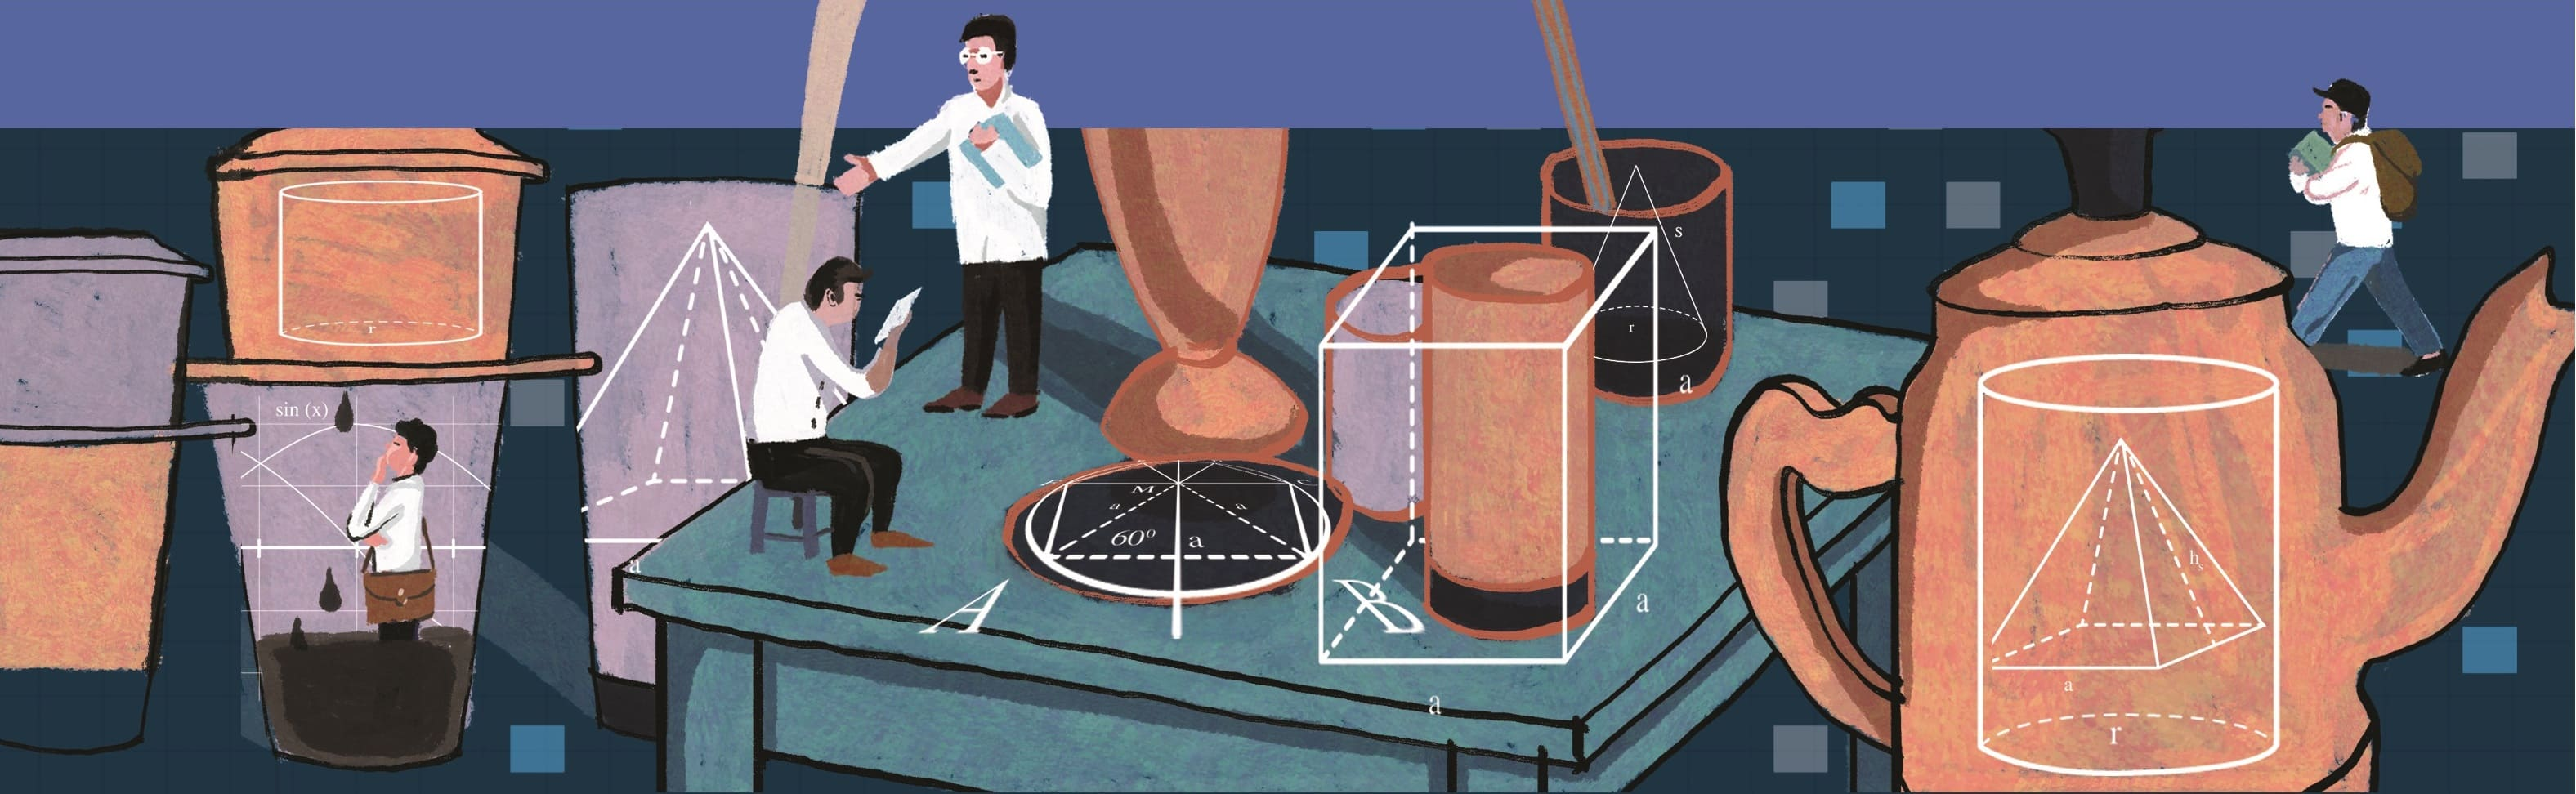
\includegraphics[width=19.3cm]{../bannerquantoan}}}
\AddToShipoutPicture*{\put(70,550){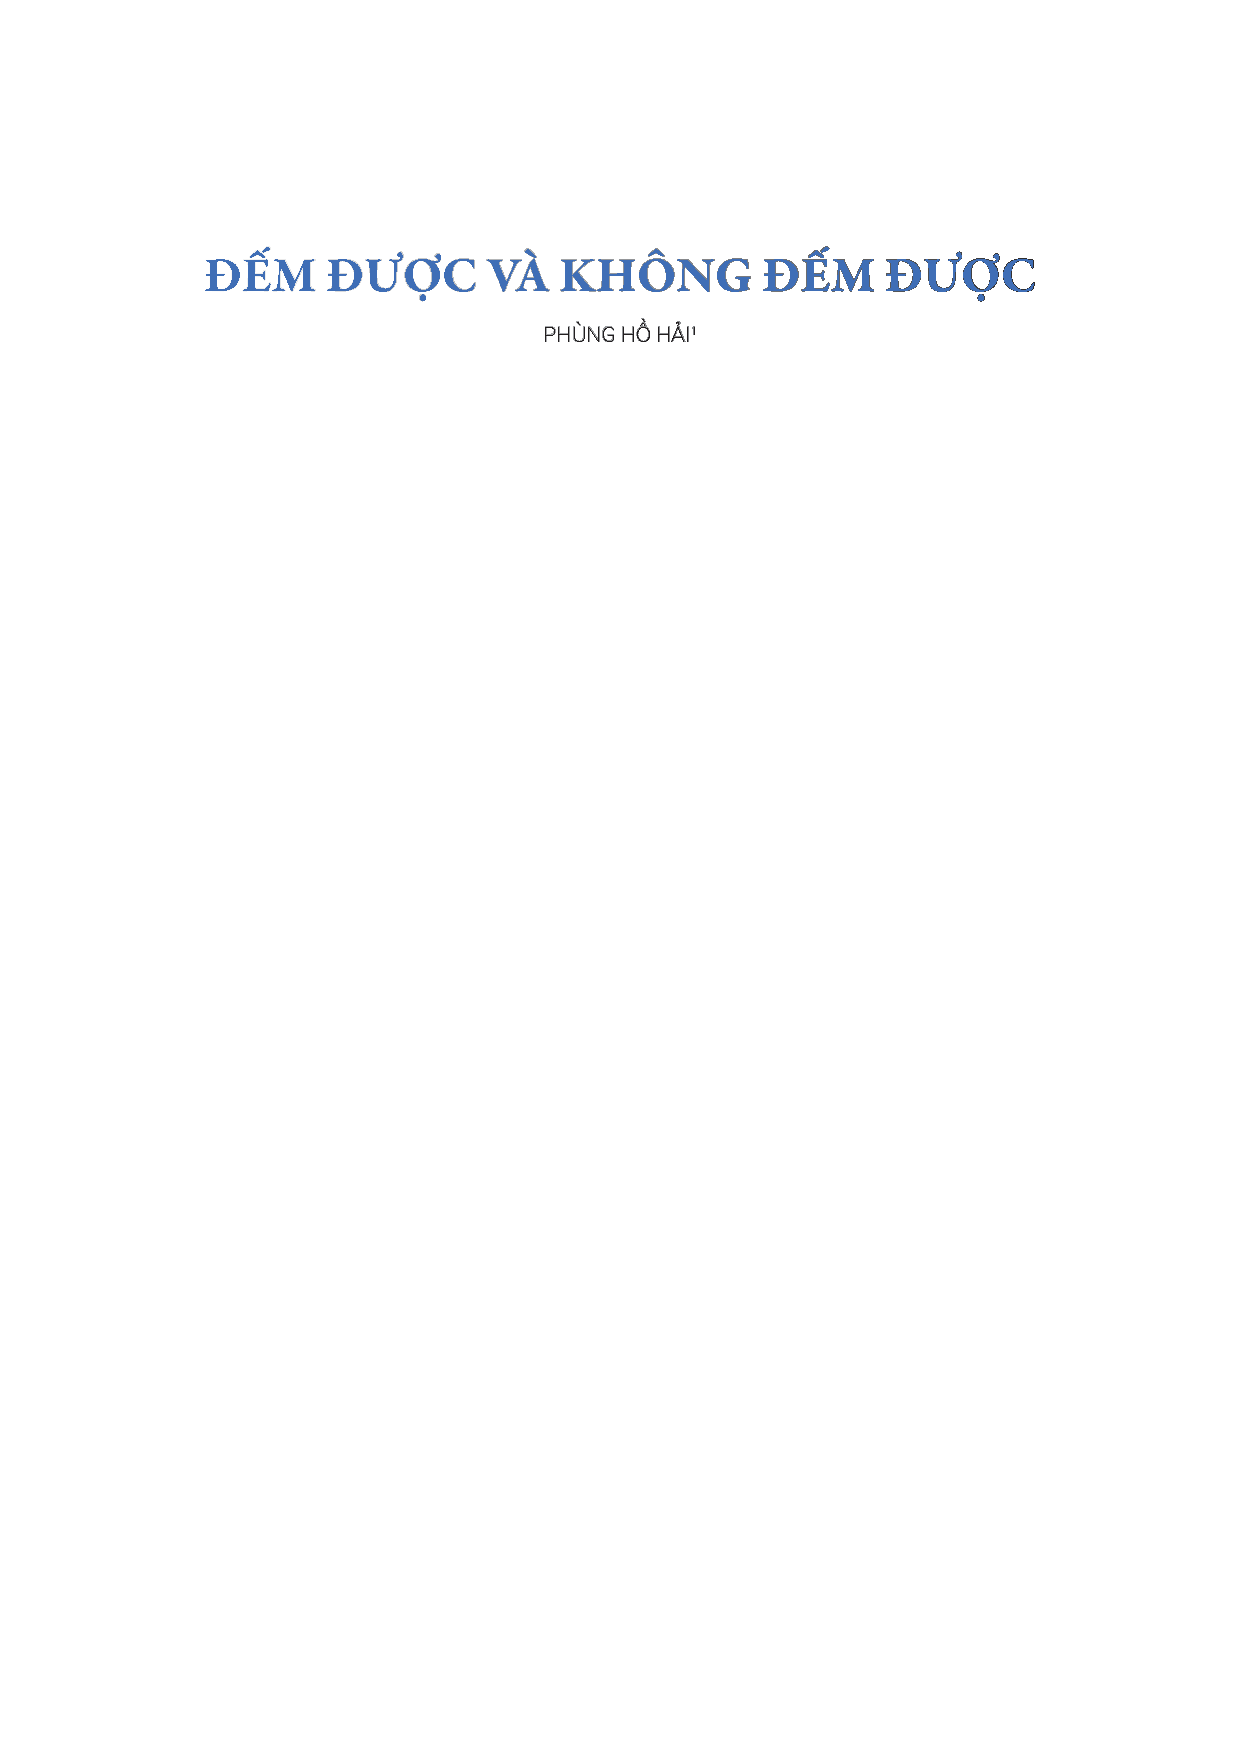
\includegraphics[scale=1]{../tieude11.pdf}}}
\centering
\endgroup

\vspace*{160pt}

\begin{multicols}{2}	
	Phép quy nạp dựa trên nguyên lý đơn giản: ta có thể tuần tự đếm được tất cả các số tự nhiên, bắt đầu từ $1$, rồi $2$, $3$, vân vân. Mặc dù ta không thể đếm được vô hạn lần, nhưng về nguyên tắc, nếu cố định một số tự nhiên, sớm hay muộn ta cũng sẽ đếm đến nó. Ta nói, tập số tự nhiên là đếm được. Bạn đọc cần phân biệt giữa ``đếm được" và ``đếm hết được nhé". Tất nhiên chúng ta không thể đếm hết được các số tự nhiên. Đếm được là cách chúng ta kiểm soát các số tự nhiên -- tuy toàn thể chúng là vô hạn, nhưng từng phần tử lại có thể đạt tới sau một quy trình hữu hạn. 
	\vskip 0.1cm
	Liệu tập các số hữu tỷ có đếm được không? Nếu hình dung các số hữu tỷ như là những điểm trên trục số, ta thấy chúng thật dày đặc. Chỉ trong khoảng giữa số $0$ và số $1$ thôi, đã có vô hạn số hữu tỷ rồi, làm sao đếm hết được!?
	\vskip 0.1cm
	Câu trả lời hóa ra là ``có" các bạn ạ. Đương nhiên, ta sẽ không đếm hết tất cả các số hữu tỷ trong khoảng $0$ đến $1$ trước rồi mới đếm tiếp các số trong khoảng $1$ đến $2$. Bởi ta không thể ``đếm hết" các số trong khoảng $0$ đến $1$. Thay vào đó, ta sẽ chọn trong mỗi khoảng một vài số để đếm dần dần, vừa ``sâu" vào trong từng khoảng đồng thời ``rộng" sang các khoảng khác. 
	\vskip 0.1cm
	Đây là một ``mẹo" rất thông minh, tác giả của nó có lẽ là Cantor. Ta sẽ biểu diễn số hữu tỷ dưới dạng phân số tối giản $\dfrac{p}{q}$, với $p$, $q$ là các số nguyên dương (để đơn giản ta sẽ chỉ đếm các số hữu tỷ dương, bạn đọc tự xây dựng cách đếm tất cả các số hữu tỷ nhé). Ta sẽ đếm dần theo cả tử số lẫn mẫu số. Bắt đầu là $\dfrac{1}{1}$, rồi $\dfrac{2}{1}$, $\dfrac{1}{2}$, rồi $\dfrac{3}{1}$, $\dfrac{1}{3}$, rồi $\dfrac{4}{1}$, $\dfrac{3}{2}$, $\dfrac{2}{3}$, $\dfrac{1}{4}$,rồi $\dfrac{5}{1}$, $\dfrac{1}{5}$, ... cứ như thế, những phân số không tối giản (ví dụ $\dfrac{2}{2}$, $\dfrac{4}{2}$,...) sẽ bị bỏ qua. Tử cùng mẫu sẽ lớn dần, tất cả các phân số tối giản sẽ được đếm, nghĩa là tất cả các số hữu tỷ (dương) sẽ được đếm. 
	\vskip 0.1cm
	Hình dung các số này trên trục số ta thấy, một mặt, các số trên khoảng $(0,1)$ sẽ được đếm ngày càng nhiều, mặt khác, mỗi bước ta lại đếm rộng ra các số trên những khoảng khác, mỗi ngày một xa. 
	\vskip 0.1cm
	Câu hỏi tiếp theo tất nhiên là về các số thực. Liệu tập số thực có đếm được không? 
	\vskip 0.1cm
	Để có thể đếm số thực, câu hỏi đầu tiên là: số thực là gì? Có lẽ các bạn ngạc nhiên bởi câu hỏi, bởi đã là số (có) thực, lại còn hỏi nó là gì! 
	\vskip 0.1cm
	Nhưng số thực là gì?
	\vskip 0.1cm
	Ta biết ví dụ về các số thực, như các số tự nhiên $1,2,3,4, \ldots$; hay các số hữu tỷ; rồi các số vô tỷ, như $\pi, e,\ldots$ Nhưng thế nào là một số thực, làm thế nào để biểu diễn một số thực?
	\end{multicols}
	\begin{figure}[H]
		\vspace*{5pt}
		\centering
		\captionsetup{labelformat= empty, justification=centering}
		
\includegraphics[width= 1\linewidth]{1a}
		\vspace*{-10pt}
	\end{figure}
	\begin{multicols}{2}
	Chúng ta sẽ thảo luận về số thực trong một bài viết sau. Để kết thúc bài viết này, tôi sẽ chỉ ra ví dụ một tập hợp không đếm được: tập các tập con của tập các số tự nhiên.
	\vskip 0.1cm
	Gọi $P_N$ là tập các tập con của tập các số tự nhiên. Như vậy, một phần tử của $P_N$ có thể là một tập hữu hạn các số tự nhiên, hoặc cũng có thể là một tập vô hạn. Thông thường ta mô tả chúng như những dãy số -- có hữu hạn hoặc vô hạn số hạng. 
	\vskip 0.1cm
	Ta sẽ chứng minh bằng phản chứng. Giả sử $P_N$ là đếm được, như vậy ta có thể sắp các phần tử của $P_N$ thành một dãy:
	\begin{align*}
		A_0, A_1, \ldots, A_k, \ldots,
	\end{align*}
	trong đó mỗi phần tử $A_k$ là một tập con của $P_N$ và mỗi tập con của $P_N$ sẽ xuất hiện như một phần tử $A_k$ ở dãy trên.
	\vskip 0.1cm
	Như vậy, với mỗi số tự nhiên $k$ sẽ có hai khả năng, hoặc nó là phần tử của $A_k$ hoặc nó không là phần tử của $A_k$. Gọi $B$ là tập hợp các số tự nhiên $k$ sao cho $k$ không là phần tử của $A_k$.
	\vskip 0.1cm
	Theo giả thiết ở trên thì $B$ sẽ xuất hiện trên dãy $(*)$ ở một vị trí nào đó, nghĩa là 
	$B=A_i$, với $i$ là một số tự nhiên nào đó.
	\vskip 0.1cm
	Các bạn có thấy điều gì vô lý không?
	Như các bạn có thể đã liên hệ với nghịch lý về sự tồn tại của ``tập tất cả các tập hợp", ở đây cũng xảy ra mâu thuẫn tương tự:
	\vskip 0.1cm
	-- $i$ không là phần tử của $B=A_i$, bởi theo giả thiết $B$ chỉ chứa những số $k$ mà $k$ không thuộc $A_k$;
	\vskip 0.1cm
	-- nếu $i$ không là phần tử của $A_i$ thì cũng theo giả thiết, $i$ thuộc $B=A_i$.
	\vskip 0.1cm
	Mâu thuẫn chứng tỏ giả thiết phản chứng của ta là sai (bạn nào chưa hiểu thế nào là chứng minh phản chứng thì xem thêm bài viết về Quy nạp nhé). Vậy ta có điều phải chứng minh: không thể liệt kê hết được các tập hợp con của tập các số tự nhiên thành một dãy, nói cách khác, tập $P_N$ các tập con của tập các số tự nhiên là không đếm được.
	\vskip 0.1cm
	Bạn đọc có thể thấy rằng chứng minh ở trên có thể lặp lại đối với một tập hợp $X$ bất kỳ để chứng minh không tồn tại một song ánh từ $X$ tới $P_X$ -- tập các tập con của $X$.
	%		\begin{figure}[H]
		%		\centering
		%		\vspace*{-5pt}
		%		\captionsetup{labelformat= empty, justification=centering}
		%		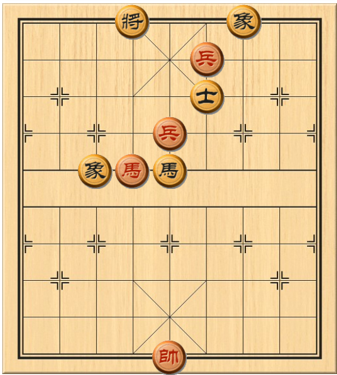
\includegraphics[width=0.5\linewidth]{4}
		%		\vspace*{-5pt}
		%	\end{figure}
\end{multicols}
%\vspace*{-10pt}
%\rule{1\linewidth}{0.1pt}
%\begin{center}
%	\textbf{\LARGE\color{quantoan}LỜI GIẢI, ĐÁP ÁN}
%\end{center}
%
%\begin{multicols}{2}
%	\textbf{\color{quantoan}Quấy rầy thám tử}
%	\vskip 0.1cm
%	Vinh và Sinh không thể cùng nói dối, như vậy trong số họ phải có một người nói thật. Vì thế Du phải là người nói dối, khi khẳng định rằng cậu ta không làm vỡ kính. Vậy người làm vỡ kính là Du.
%	\vskip 0.1cm
%	\textbf{\color{quantoan}Đố vui}
%	\vskip 0.1cm
%	Đánh số các quả cân từ $1$ đến $6$. 
%	\vskip 0.1cm
%	Trước hết cân $1$ với $2$. Giả sử chúng nặng bằng nhau. Ở lần cân thứ hai, ta cân $1$ với $3$. Nếu chúng nặng bằng nhau thì $1$, $2$, $3$ là các quả cân nặng bằng nhau (cũng như $4$, $5$ và $6$). Do đó ở lần cân thứ $3$ ta chỉ cần so sánh $1$ và $4$ để xác định được những quả cân nào là đúng và những quả cân nào là sai. Nếu không, chẳng hạn $1$ nặng hơn $3$ (trường hợp $1$ nhẹ hơn $3$ tương tự), thì các quả cân $1$ và $2$ là các quả cân đúng và quả cân $3$ là quả cân sai. Bây giờ, trong số các quả cân $4$, $5$, $6$ có một quả cân đúng và hai quả cân sai. Để xác định, ta chỉ cần cân $4$ với $5$: nếu chúng nặng bằng nhau thì nghĩa là $4$ chúng là các quả cân sai; nếu không, quả nặng hơn là quả cân đúng (còn hai quả còn lại là quả cân sai). 
%	\vskip 0.1cm
%	Bây giờ, giả sử $1$ nặng hơn $2$ (trường hợp ngược lại tương tự), nghĩa là quả cân $1$ là đúng và quả cân $2$ là sai. Ở lần cân thứ hai, ta cân $1$ với $3$ để xác định được $3$ là quả cân đúng hai sai. Như vậy, sau $2$ lần cân, ta xác định được ba quả cân $1$, $2$, $3$: gồm hai quả đúng và một quả sai hoặc hai quả sai và một quả đúng. Ở lần cân cuối cùng, ta tiến hành như ở trường hợp bên trên, bằng cách cân $4$ với $5$, để xác định được những quả cân nào đúng và quả cân nào sai.  
%	\vskip 0.1cm
%	\hfill(\textit{Xem tiếp trang $36$})	
%		\textbf{Góc cờ}
%		\vskip 0.1cm
%		Hình $4$: $\pmb{1)}$	M$6.7$ Tg$4.1$\quad $\pmb{2)}$ C$5-6$ M$5.3$\quad $\pmb{3)}$ M$7/5$ Tg$4/1$\quad $\pmb{4)}$ C$6.1$ Tg$4-5$\quad $\pmb{5)}$ Tg$5-4$ T$7.9$\quad $\pmb{6)}$ C$6.1$ M$3.4$\quad $\pmb{7)}$ M$5.7$ ($1-0$)
%		\vskip 0.1cm
%		Hình $5$: $\pmb{1)}$ X$1-5$ M$8/7$\quad $\pmb{2)}$ X$5.1$ Tg$5/1$\quad $\pmb{3)}$ X$5-3$ Tg$5-4$\quad $\pmb{4)}$ X$3-6$ Tg$4-5$\quad $\pmb{5)}$ X$6.1$ Tg$5.1$\quad $\pmb{6)}$ X$6-8$ Tg$5-4$\quad $\pmb{7)}$ X$8.1$ Tg$4/1$\quad $\pmb{8)}$ X$8-5$ ($1-0$)
%\end{multicols}